% (C) Copyright 2016
% Urs Fässler, www.bitzgi.ch
% SPDX-License-Identifier: CC-BY-SA-4.0

\section{Teaser}
{
\usebackgroundtemplate{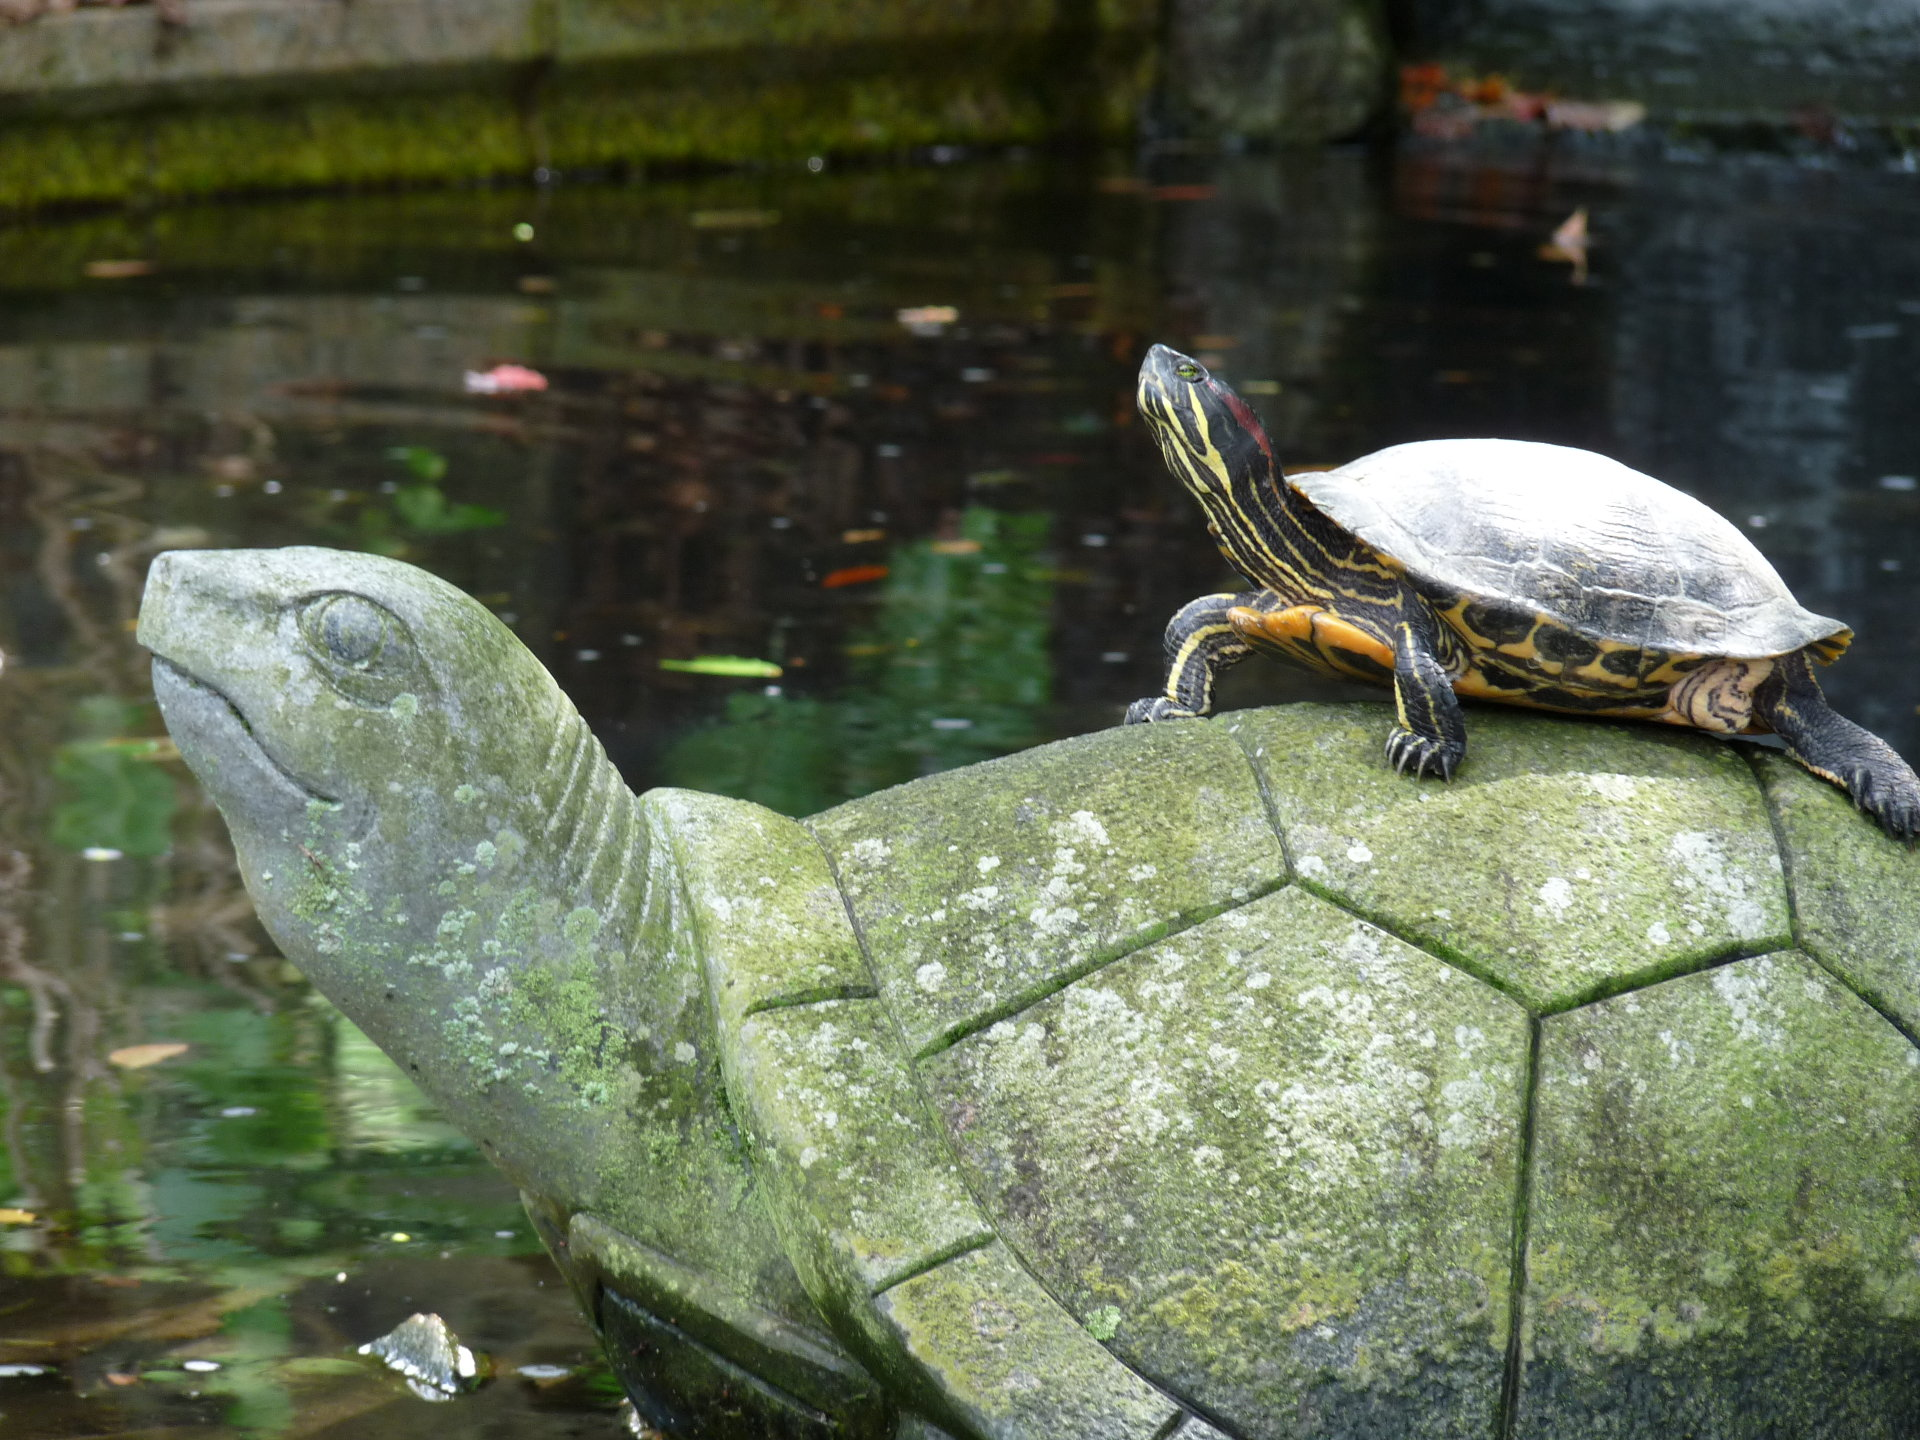
\includegraphics[height=\paperheight,width=\paperwidth]{res/turtles.jpg}}
\begin{frame}[plain]
	\begin{center}
		\color{white}
		\Large
		\visible<2->{\textbf{\textcopyright}\ }\visible<3->{Urs Fässler}\visible<4->{ CC-BY-SA}
		\vspace{0.8\paperheight}
	\end{center}
\end{frame}
\note{
	\begin{itemize}
		\item eigenes Foto
		\item habe ich das Copyright drauf?
		\item darf es kopiert und verwendet werden?
		\item ändert das Copyright Zeichen und Name etwas?
		\item ändert ein CC-BY-SA etwas?
		\item \url{http://hoesmann.eu/rechtsgebiete/urheberrecht/faq-foto-und-urheberrecht/}
	\end{itemize}
}

\section{Thema}
\note{
	\begin{itemize}
		\item Eine Einführung in die Lizenzen der Freien Software (Open Source)
	\end{itemize}
}

\section{Behauptung}
\note
{
	\begin{itemize}
		\item Korrekte Verwendung Freier Software ist nicht schwer
	\end{itemize}
}

}
